\documentclass[handout]{beamer}

\usetheme[progressbar=frametitle]{metropolis}
\usepackage{appendixnumberbeamer}
\usepackage{booktabs}
\usepackage{amsmath}
\usepackage{amssymb}
\usepackage{tcolorbox}
\usepackage{tikz}

\definecolor{metropolisblue}{RGB}{39, 59, 94}



% Begin document
\begin{document}

% Title page
\title{Monte Carlo Methods}
\subtitle{Univariate}
\author{Nipun Batra}
\date{\today}
\institute{IIT Gandhinagar}
\maketitle

% Section 1
\section{Introduction}

\begin{frame}{General Form}
The general form of Monte Carlo methods is:
\begin{equation}
    \mathbb{E}[f(X)] = \int f(x) p(x) dx \approx \frac{1}{N} \sum_{i=1}^N f(x_i)
\end{equation}
where $x_i \sim p(x)$.
\end{frame}
\begin{frame}[fragile]{Estimating Pi using Monte Carlo (Part 1)}
    We can estimate the value of pi using Monte Carlo methods by considering a unit square with a quarter circle inscribed within it.
    
    \begin{itemize}
        \item Let $p(x)$ be defined over the unit square using the uniform distribution in two dimensions, i.e., $p(x) = 1$ for $x \in [0, 1]^2$.
        \item Let $f(x)$ be the indicator function defined as follows:
            \[
            f(x) = \begin{cases}
                        \text{\textcolor{green}{Green}} (1), & \text{if } x \text{ falls inside the quarter circle}, \\
                        \text{\textcolor{red}{Red}} (0), & \text{otherwise}.
                   \end{cases}
            \]
    \end{itemize}
    
    \begin{center}
    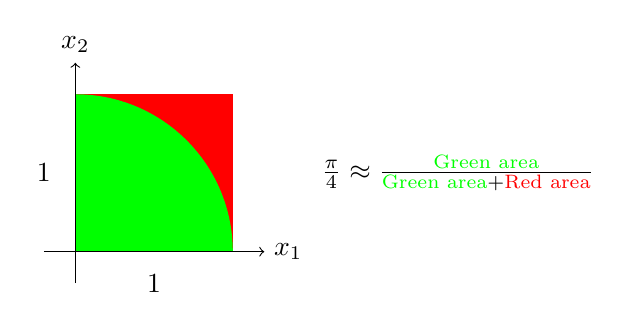
\begin{tikzpicture}[scale=2]
        % Unit Square
        \fill[red] (0,0) rectangle (1,1);
        
        % Quarter Circle
        \fill[green] (0,0) -- (0,1) arc (90:0:1) -- cycle;
        
        % Coordinate Axes
        \draw[->] (-0.2,0) -- (1.2,0) node[right] {$x_1$};
        \draw[->] (0,-0.2) -- (0,1.2) node[above] {$x_2$};
        
        % Labels
        \node at (0.5, -0.2) {1};
        \node at (-0.2, 0.5) {1};
        \node[right] at (1.5, 0.5) {$\frac{\pi}{4} \approx \frac{\text{\textcolor{green}{Green area}}}{\text{\textcolor{green}{Green area}} + \text{\textcolor{red}{Red area}}}$};

    \end{tikzpicture}
    \end{center}
    \end{frame}
    

\end{document}